%\newpage
%\section{Introduction}

Up to now, we have known that machine learning algorithms can be used to effectively learn a function $f$ from a set of input-output pairs. The function $f$ approximates the relation between two random variables $X$ and $Y$, and actually expresses the conditional probability $P_f(Y|X)$. However, in a complex, real world system, there might be more than two random variables and it is useful to not only understand the the conditional probability between random variables but also be able to infer more intriguing information from the conditional dependence relations between random variables.
It is also possible that, a complex machine learning model, such as a convolutional neural network, can be approximated by constructing the conditional dependencies between a set of random variables representing the features learned by the neural networks, see e.g., \cite{berthier2021abstraction} for an example.  Therefore, while it is agreeable that machine learning has been able to support human operators in dealing with some long-standing tasks such as object detection and recognition with accuracy and efficiency, there is still a need to infer useful knowledge from a set of conditional probabilities. 
This chapter is to explain how we may utilise probabilistic graphical model, a formalism to express conditional probabilities between random variables ($X$, $Y$, and variables for latent representations), as an abstract model for neural network. We will present the definition in Section~\ref{sec:defPGM} and then discuss the abstraction method in Section~\ref{chap:NNabstraction}. More detailed introduction to probabilistic graphical models is given in the Appendix (Chapter~\ref{chap:pgm}). 

\section{Definition of Probabilistic Graphical Models}\label{sec:defPGM}

Probabilistic graphical models are a formalism for the above purpose. They use a structure, or more specifically a graph, to represent conditional dependence relations between random variables, and use a probability table for every random variable to express the local dependence relation of the random variable. There are two major branches of graphical models, namely, Bayesian networks and Markov random fields, and in this chapter, we focus on Bayesian network. In the following, we will use (probabilistic) graphical models and Bayesian network interchangeably. 


Depending on the dependence relation of individual random variable, the probability tables in a graphical model can be a marginal probability table, which shows that the random variable does not depend on any other variables in the graph, or a conditional probability table, which represents the conditional probability distribution of the current random variable over other random variables in the graph. 

\begin{figure}[!htbp]
    \centering
    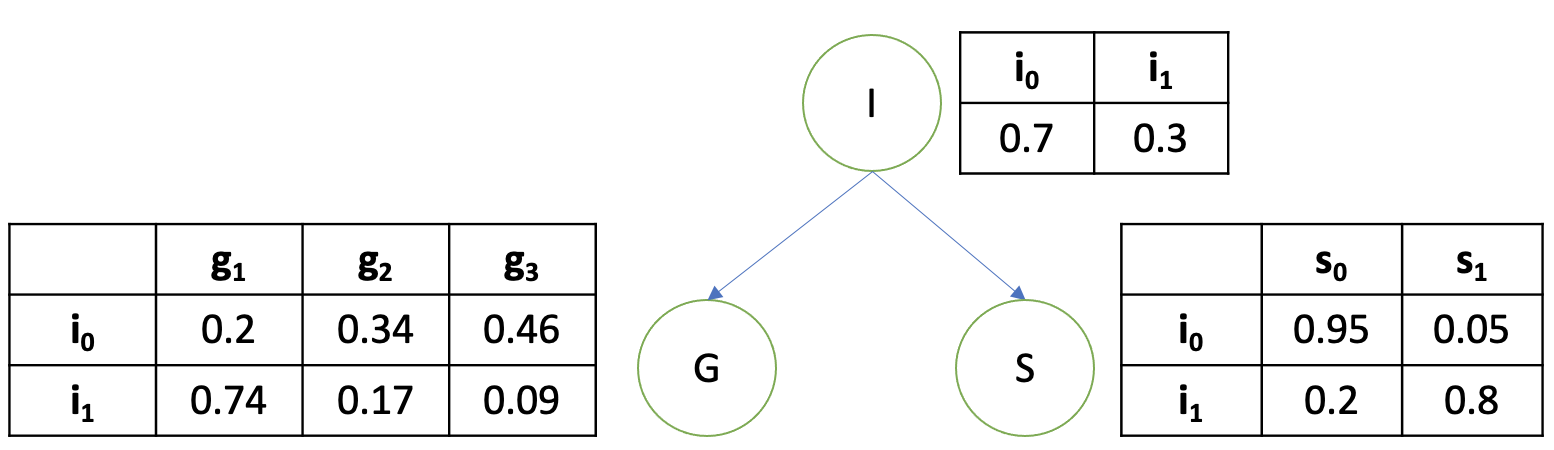
\includegraphics[width=0.7\textwidth]{images/graphical models/threeNodes.png}
    \caption{A simple graphical model of three nodes}
    \label{fig:threeNodes}
\end{figure}


Figure~\ref{fig:threeNodes} presents a simple graphical model with 3 nodes: $I, G, S$. We can see that one of the nodes $I$ has a marginal probability table while the remaining two nodes have conditional probability tables. 
Summarising, 
\begin{equation}
    \text{Probabilistic Graphical Model = Graphical Structure + Multivariate Statistics}
\end{equation}
Formally, a probabilistic graphical model $G=({\cal V},{\cal E},P)$ where ${\cal V}$ is a set of nodes, representing the random variables, ${\cal E}$ is the set of edges between nodes, and $P$ is a set of probability tables, one for each node in ${\cal V}$. 

\section*{A Running Example}

Assume that, on a self-driving car, there are two sensors, $Camera$ and $Radar$, that are used to detect pedestrian collectively. The precision of the  camera may be affected by weather conditions, such as the $Fog$ as we consider in this example. The $Radar$ may be affected by the distance of the object from the car, i.e., it can be very precise when the object is close but may become less precise when the object is $Away$. Once a pedestrian is detected and it is not away, the car will need to stop. 

%\begin{example}


\begin{figure}[!htbp]
    \centering
    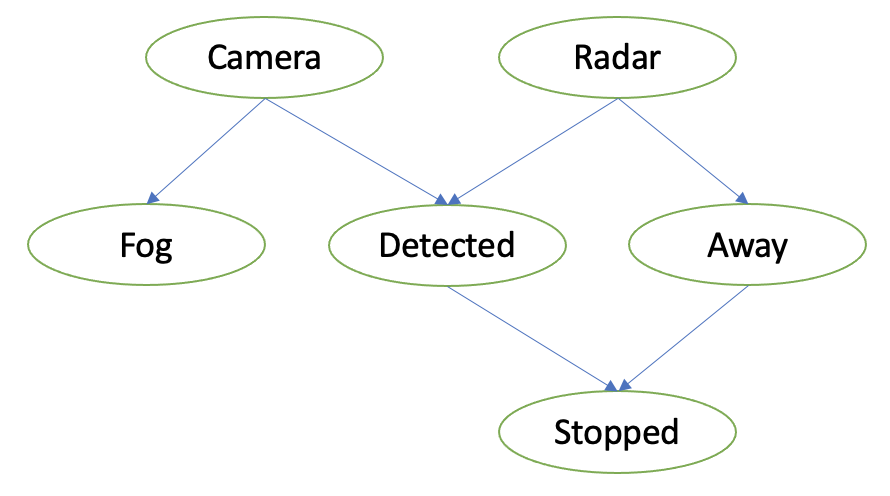
\includegraphics[width=0.6\textwidth]{images/graphical models/graphicalmodel.png}
    \caption{A simple Bayesian network for safety analysis on vehicle stopping upon pedestrian detection}
    \label{fig:graphicalmodel}
\end{figure}

Figure~\ref{fig:graphicalmodel} presents a probabilistic graphical model for this example. In the graph $G$, there are six random variables: $Camera$, $Radar$, $Fog$, $Detected$, $Away$, and $Stopped$. Every node is associated with either a marginal probability table or a conditional probability table, depending on whether they have incoming edges. The information about the probability tables are given in Figure~\ref{fig:cameratables}. For example, the nodes $Camera$ and $Radar$ do not have incoming edges, so each of them is associated with a marginal probability table. Intuitively, the two tables suggest that the probability of a pedestrian appearing in the imagery input of the camera is $0.4$, and in the signal input of the radar is $0.5$. Note that, the ``appearing'' is for ground truth (through human's eyes), not for the result of a detection system. The detection is implemented through the $Detected$ node to be explained below. 


%\end{example}


\begin{figure}[!htbp]
    \centering
    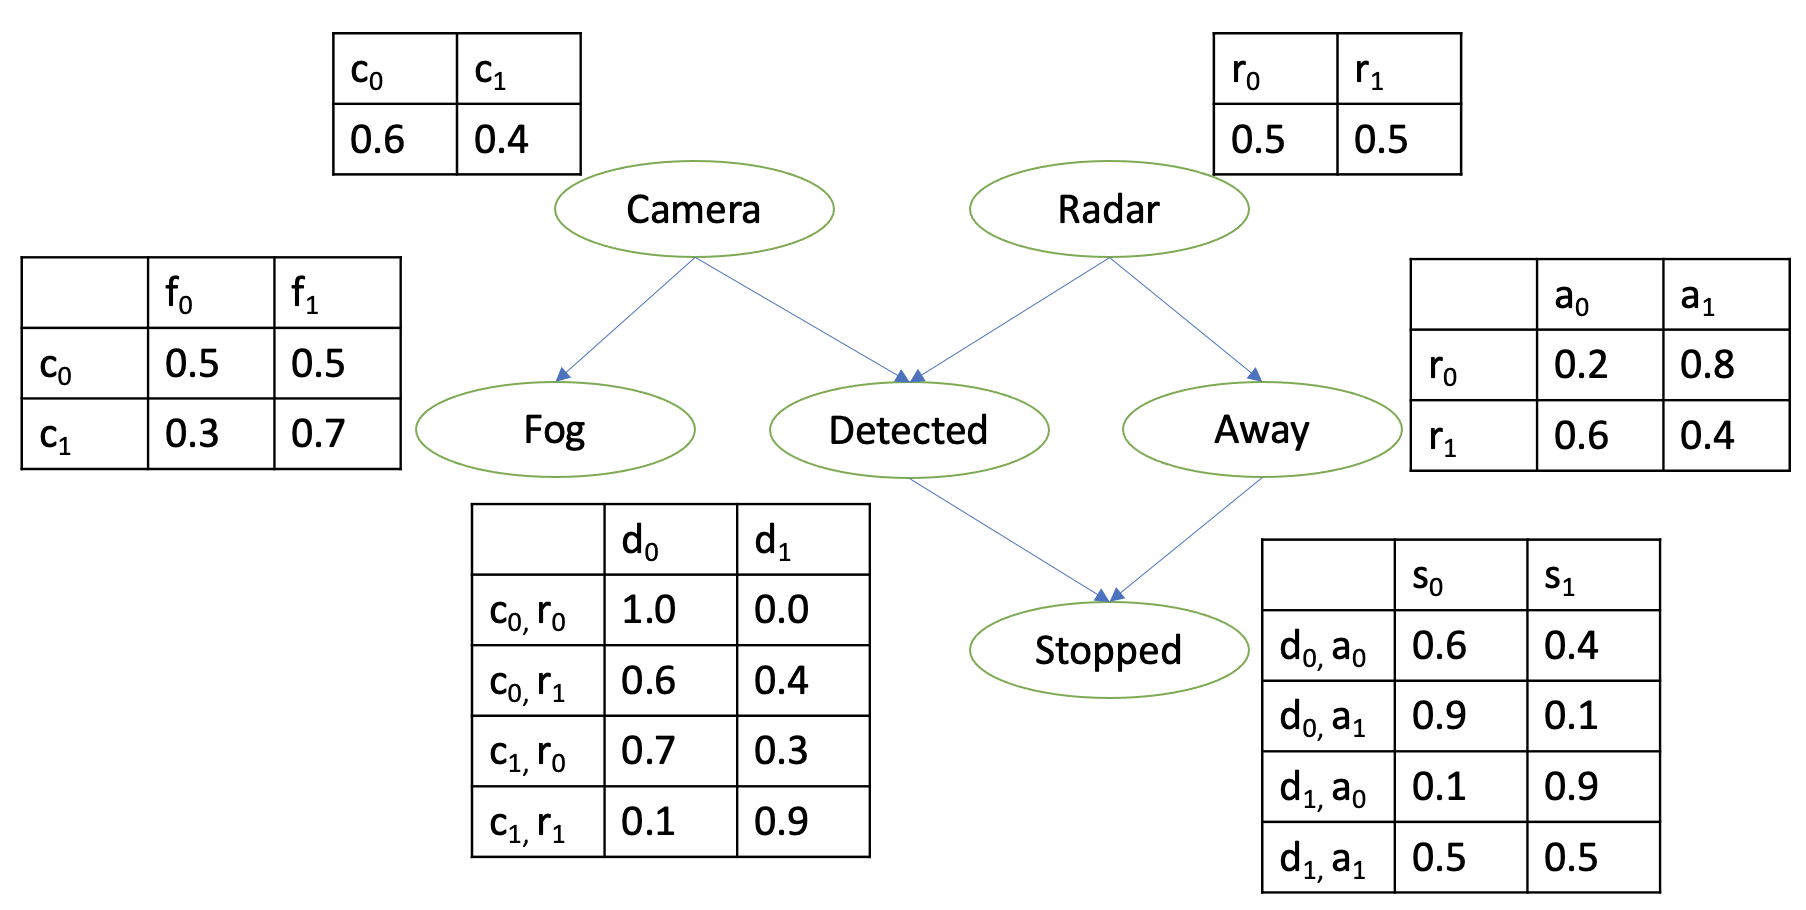
\includegraphics[width=\textwidth]{images/graphical models/cameramodel.png}
    \caption{Probabilistic table of the graphical model in Figure~\ref{fig:graphicalmodel}}
    \label{fig:cameratables}
\end{figure}


Other nodes are associated with conditional probability tables. For example, the table for $Fog$ shows that, when there is no pedestrian appearing in the imagery input, the probability of the foggy weather condition is $0.5$.  This probability is lowered when there is a pedestrian appearing in the imagery input. This is intuitive, because the foggy condition may affect the ability of camera capturing the pedestrian. Similar for the $Away$ node. When there is no pedestrian appearing in the signal input, the probability of its away from a pedestrian is $0.8$. This probability is lowered to $0.4$ when there is a pedestrian appearing in the signal input. 

The detection result is a fusion of both camera and radar's results. Note that, even if a pedestrian appears in the imagery input, it does not mean that the pedestrian can be detected (Recall the generalisation error and robustness error of deep learning). We note that, if neither of the sensors has a pedestrian appeared, no detection can be made at all. If one of the sensors has a pedestrian, there is a non-trivial chance that it can be detected. The detection becomes significantly better when both sensors captured the pedestrian. 

Finally, the decision making on whether the car should be stopped is based on both the detection result and the distance. If it is detected (i.e., $Detected = d_1$) and not far away (i.e., $Away = a_0$) then this probability is high ($0.9$). Otherwise, the probability is low ($0.1$). The lowest probability appears when no pedestrian is detected (i.e., $Detected = d_0$) and it is away (i.e., $Away = a_1$). 

\subsection*{Where does machine learning play a role?}

Machine learning can be used to generate those conditional probability tables. For example, a deep learning model can be designed and trained to get the table for $Detected$ node, i.e., classify whether a pedestrian is detected or not on both the camera input and the radar input. Similarly, other nodes such as $Fog$, $Away$, and $Stopped$ may also be implemented with a machine learning model. 

